\section{Deep model evaluation}
\label{sec:Deep model evaluation}
Due to the relatively short period for data collection in this study, from the beginning of 2021 June to the end of July, the total size of validly labelled videos collected was approximately 440MB.
By decoding these videos and videos randomly selected from the public data set Kinetics as the Unknown category into images, the total size of these images is approximately 2.3GB.

\begin{figure}[!ht]
    \centering
    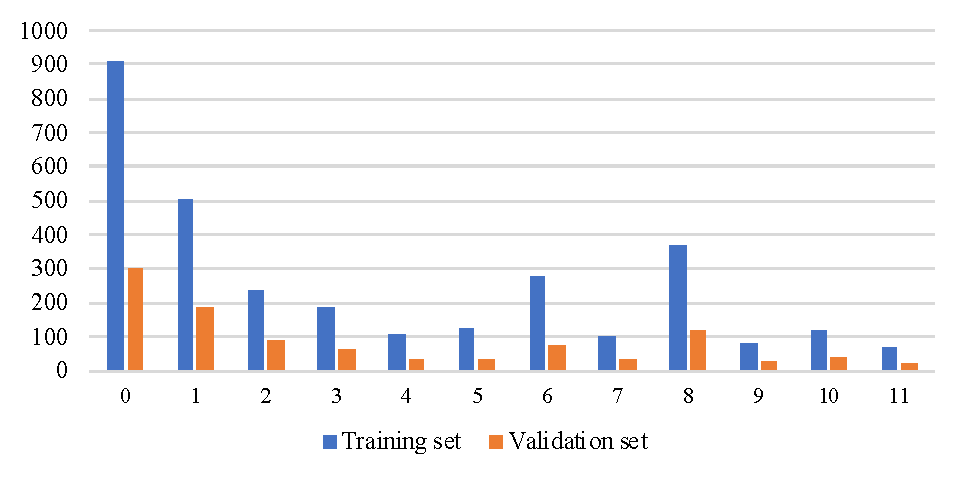
\includegraphics[width=\textwidth]{evaluation/imgs/5-data-dist-diag.pdf}
    \caption{Data per category distribution}
    \label{fig:5-data-dist-diag}
\end{figure}

Figure \ref{fig:5-data-dist-diag} shows the per-category data distribution after dividing the anonymised data into training and validation sets.
The horizontal axis of the histogram shows a total of 12 categories from 0 to 11.
Table \ref{tab:Model output} in the model design chapter introduced the definition of each category.
As for the vertical axis, it represents the number of labelled samples.
A labelled sample has one label and 16 frames from temporal sampling in a video clip.
To ensure that the validation data set has enough samples to illustrate the model performance, one-third of the total data set is divided into the validation data set, and the remaining two-thirds are used for training the deep model.

Over-fitting is an unavoidable problem in deep learning, especially when using a complex model on small data sets.
It is a phenomenon that the model loses its generalisation application ability, which manifests as the model has extremely small loss and very high accuracy on the training set, however, a over-fitted model will perform badly on the validation set. 
The main reasons for over-fitting and the corresponding solutions are as follows:
\begin{enumerate}
    \item The size of the data set does not match the complexity of the model. \\ \textbf{Solution}: To use data augmentation or reduce the model complexity.
    \item There are errors in the data sets, e.g. data have wrong labels, unshuffled data resulting in distribution difference between the training set and the validation set. \\
    \textbf{Solution}: To visually inspect the data sets and ensure reliable data set labelling and distribution.
    \item Over-training, the model has been trained too much. \\
    \textbf{Solution}: To reduce the number of training epochs or use the early-stop mechanism to detect increasing loss in the validation set.
\end{enumerate}

In this study, the above three solutions were all applied in the training process to avoid over-fitting.
In detail, the early-stop mechanism is implemented the model trainer, which monitors the loss value on the verification set after each training epoch.
Once the verification loss is found to increase, it will stop training.
The data loader uses common data augmentation methods in computer vision to perform the same transformation on the same batch of input data, such as scaling, randomly cropping, and flipping horizontally and vertically.
Besides, the data sets are carefully validated and visually checked using Jupyter notebook with \textit{matplotlib.animation} library.

\begin{figure}[!ht]
    \centering
    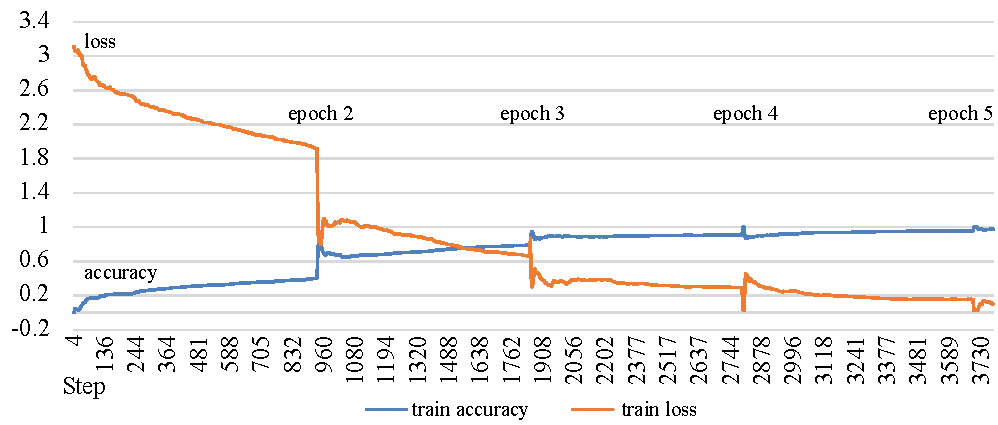
\includegraphics[width=.85\textwidth]{evaluation/imgs/5-train-step.pdf}
    \caption{Model training steps}
    \label{fig:5-train-step}
\end{figure}
\begin{figure}[!ht]
    \centering
    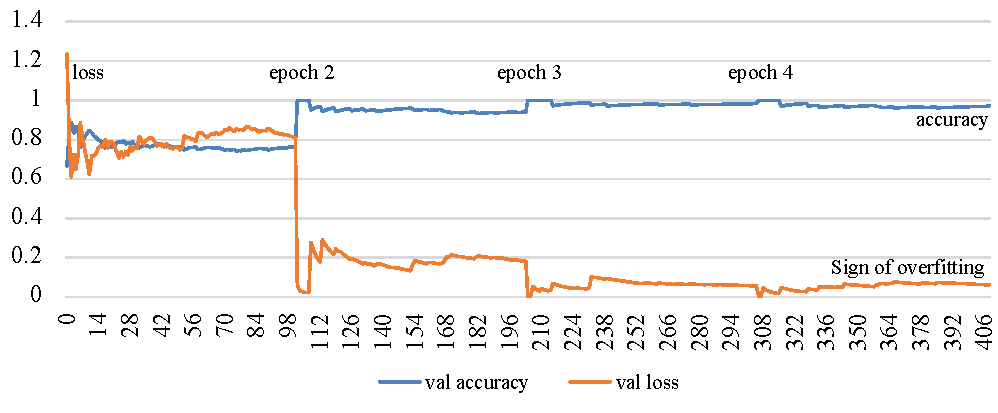
\includegraphics[width=.85\textwidth]{evaluation/imgs/5-val-steps.pdf}
    \caption{Model validation steps}
    \label{fig:5-val-steps}
\end{figure}

Figure \ref{fig:5-train-step} and Figure \ref{fig:5-val-steps} display the model training and validating iterations.

\clearpage
\begin{figure}[H]
    \centering
    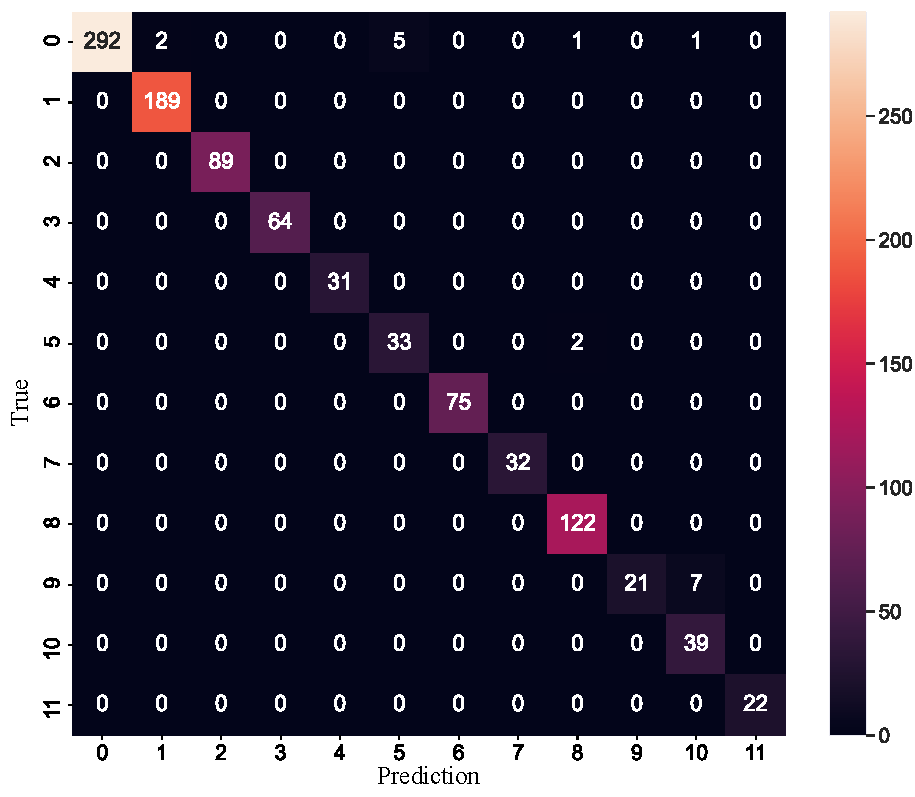
\includegraphics[width=.74\textwidth]{evaluation/imgs/5-confusion_matrix_val.pdf}
    \caption{Confusion matrix on validation data set}
    \label{fig:5-confusion_matrix_val}
\end{figure}

\begin{figure}[H]
    \centering
    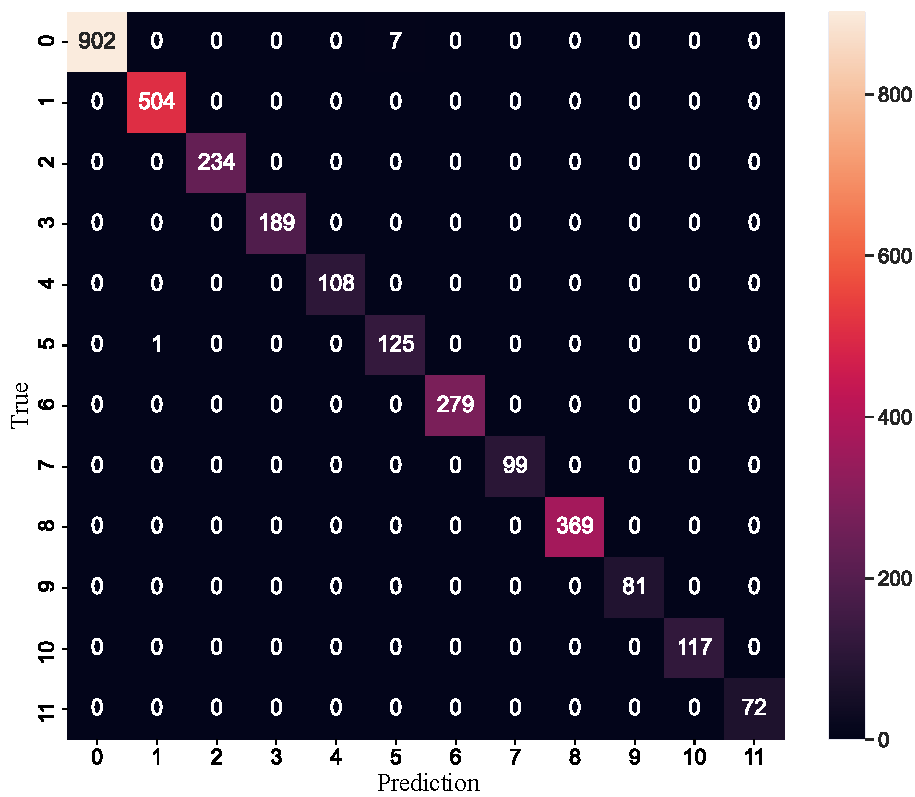
\includegraphics[width=.74\textwidth]{evaluation/imgs/5-confusion_matrix_train.pdf}
    \caption{Confusion matrix on training data set}
    \label{fig:5-confusion_matrix_train}
\end{figure}

\begin{table}[!htbp]
\centering
\begin{tabular}{|l|c|c|c|c|}
\hline
              & Precision & Recall & F1-Score & Support \\ \hline
0 Unknown     & 1.00      & 0.97   & 0.98     & 301     \\ \hline
1 Look screen & 0.99      & 1.00   & 0.99     & 189     \\ \hline
2 Look down   & 1.00      & 1.00   & 1.00     & 89      \\ \hline
3 Look side   & 1.00      & 1.00   & 1.00     & 64      \\ \hline
4 Look back   & 1.00      & 1.00   & 1.00     & 31      \\ \hline
5 Leave       & 0.87      & 0.94   & 0.90     & 35      \\ \hline
6 Speaking    & 1.00      & 1.00   & 1.00     & 75      \\ \hline
7 Look up     & 1.00      & 1.00   & 1.00     & 32      \\ \hline
8 Use phone   & 0.98      & 1.00   & 0.99     & 122     \\ \hline
9 Scratching  & 1.00      & 0.75   & 0.86     & 28      \\ \hline
10 Drinking   & 0.83      & 1.00   & 0.91     & 39      \\ \hline
11 Typing     & 1.00      & 1.00   & 1.00     & 22      \\ \hline
Accuracy      & \multicolumn{3}{c|}{0.98}     & 1027    \\ \hline
macro avg     & 0.97      & 0.97   & 0.97     & 1027    \\ \hline
weighted avg  & 0.98      & 0.98   & 0.98     & 1027    \\ \hline
\end{tabular}
\caption{Test classification report on validation data set}
\label{tab:Test classification report}
\end{table}
